\documentclass[a4paper,11pt]{article}
\usepackage[english,russian]{babel}
\usepackage[utf8]{inputenc}
\usepackage{a4wide}
\usepackage{amsmath}
\usepackage{float}
\usepackage{graphicx}
\usepackage{longtable}
\input PATTERN.TEX
\input OPR.TEX

\begin{document}

\section{Постановкa дифференциальной задачи}
Система уравнений, описывающая нестационарное движение баротропного газа
в области $\Omega$,
выглядит следующим образом
\begin{equation}
\begin{array}{l}
\dfrac{\partial \rho}{\partial t}+\dfrac{\partial \rho u_1}{\partial x_1}+
\dfrac{\partial \rho u_2}{\partial x_2}= 0, \\[2.0ex]
\dfrac{\partial \rho u_1}{\partial t}
+\dfrac{\partial \rho u_1^2}{\partial x_1}+
\dfrac{\partial \rho u_2 u_1}{\partial x_2}+
\dfrac{\partial p}{\partial x_1}
=\mu\left(
\dfrac{4}{3}\dfrac{\partial^2 u_1}{\partial x_1^2}+
\dfrac{\partial^2 u_1}{\partial x_2^2}+
\dfrac{1}{3}\dfrac{\partial^2 u_2}{\partial x_1\partial x_2}\right)
+\rho f_1, \\[2.0ex]
\dfrac{\partial \rho u_2}{\partial t}
+\dfrac{\partial \rho u_1 u_2}{\partial x_1}+
\dfrac{\partial \rho u_2^2}{\partial x_2}+
\dfrac{\partial p}{\partial x_2}
=\mu\left(
\dfrac{1}{3}\dfrac{\partial^2 u_1}{\partial x_1\partial x_2}+
\dfrac{\partial^2 u_2}{\partial x_1^2}+
\dfrac{4}{3}\dfrac{\partial^2 u_2}{\partial x_2^2}\right)
+\rho f_2,
\end{array}
\label{dif.1}
\end{equation}

Неизвестные функции: плотность $\rho$  и вектор скорости $\u$ являются
функциями переменных Эйлера
$$
(t,\x) \in Q=[0,T]\times\bar\Omega.
$$%

Обозначим через $\Omega_{nm}$ квадрат, координаты точек которого удовлетворяют
неравенствам $n < x < (n+1)$ и $m < y < (m+1)$. Множества точек,
составляющие стороны квадрата $\Omega_{nm}$ обозначим $\Gamma_{nm}^{x-}$,
$\Gamma_{nm}^{x+}$, $\Gamma_{nm}^{y-}$ и $\Gamma_{nm}^{y+}$,
где индекс $x$ или $y$ означает какая из координат на стороне
является постоянной,
а + или - означает максимальное или минимальное значение
принимает эта координата.

Заданная область: 9. $\bar\Omega=\bar\Omega_{01}\cup\bar\Omega_{02}\cup\bar\Omega_{11}\cup
\bar\Omega_{12}\cup\bar\Omega_{20}\cup\bar\Omega_{21}\cup\bar\Omega_{22}$,

Граничные условия для неизвестного решения: $u_1\vert_{\Gamma_{01}^{x-}\cup\Gamma_{02}^{x-}}=w$,
$\frac{\partial u_2}{\partial y}\vert_{\Gamma_{20}^{y-}}=0$.
На остальных участках границы
функция плотности считается неизвестной и подлежит определению, а компоненты функции скорости равны нулю.









\newpage
\section{Схема А.Г.Соколова ПЛОТНОСТЬ-СКОРОСТЬ}
\label{r_v_sok}

Сеточная функция $\V$, приближающая функцию вектора скорости $\u$, определяется
в узлах сетки $\bar Q_{\tau\bar h}$, а значения функции $H$, приближающей
функцию плотности $\rho$, ищутся в узлах сетки $Q^{1/2}_{\tau\bar h}$ по
следующей схеме, аппроксимирующей систему~(\ref{dif.1})

\begin{equation}
\begin{array}{l}
H_t+(\sigma_1\{\hat H,{V_1}_{s_2}\} {V_1}_{s_2})_{x_1}
+(\sigma_2\{\hat H,{V_2}_{s_1}\} {V_2}_{s_1})_{x_2}=0,
\qquad \x\in\Omega^{1/2}_{\bar h};\\
\hat H_{\bar s_1\bar s_2}{V_1}_t+
\hat H_{\bar s_1\bar s_2} \delta_1\{\hat V_1,V_1\}+
\hat H_{\bar s_1\bar s_2} \delta_2\{\hat V_1,V_2\}
+p(\hat H_{\bar s_2})_{\bar x_1}=\\
=\mu\left(\frac{4}{3}(\hat V_1)_{x_1\bar x_1}+(\hat V_1)_{x_2\bar x_2}\right)+
\dfrac{\mu}{3}(V_2)_{\xo_1\xo_2}+f_1\hat H_{\bar s_1\bar s_2},
\qquad \hbox{при}\; \hat H_{\bar s_1\bar s_2}\ne 0,\\
\hat V_1=0, \qquad \hbox{при}\; \hat H_{\bar s_1\bar s_2}=0,
\qquad \x\in\Omega_{\bar h};\\
\hat H_{\bar s_1\bar s_2}{V_2}_t+
\hat H_{\bar s_1\bar s_2} \delta_1\{\hat V_2,V_1\}+
\hat H_{\bar s_1\bar s_2} \delta_2\{\hat V_2,V_2\}
+p(\hat H_{\bar s_1})_{\bar x_2}=\\
=\mu\left((\hat V_2)_{x_1\bar x_1}+\frac{4}{3}(\hat V_2)_{x_2\bar x_2}\right)+
\dfrac{\mu}{3}(V_1)_{\xo_1\xo_2}+f_2\hat H_{\bar s_1\bar s_2},
\qquad \hbox{при}\; \hat H_{\bar s_1\bar s_2}\ne 0,\\
\hat V_2=0, \qquad \hbox{при}\; \hat H_{\bar s_1\bar s_2}=0,
\qquad \x\in\Omega_{\bar h}.
\end{array}
\label{r_v_sok.1}
\end{equation}

В граничных узлах $\gamma_{\bar h}$ значения функции $\V$ считаются известными
из граничных условий. В граничных узлах, где газ втекает в область, задаются
значения плотности газа, которые также берутся из граничных условий.

Разностные уравнения в индексах имеют вид:
\begin{equation}
\begin{array}{c}
\dfrac{H^{n+1}_{m_1,m_2}-H^n_{m_1,m_2}}{\tau}+\\
+\dfrac{
(({{\tilde V}_2})^n_{m_1,m_2+1}-|({{\tilde V}_2})^n_{m_1,m_2+1}|)H_{m_1,m_2+1}^{n+1}
}{2h_2}
+\dfrac{
(({{\tilde V}_1})^n_{m_1+1,m_2}-|({{\tilde V}_1})^n_{m_1+1,m_2}|)H_{m_1+1,m_2}^{n+1}
}{2h_1}+ \\
+\left(\dfrac{1}{2h_1}
(({{\tilde V}_1})^n_{m_1+1,m_2}+|({{\tilde V}_1})^n_{m_1+1,m_2}|
-({{\tilde V}_1})^n_{m_1,m_2}+|({{\tilde V}_1})^n_{m_1,m_2}|)+\right.\\
\left.+\dfrac{1}{2h_2}
(({{\tilde V}_2})^n_{m_1,m_2+1}+|({{\tilde V}_2})^n_{m_1,m_2+1}|
-({{\tilde V}_2})^n_{m_1,m_2}+|({{\tilde V}_2})^n_{m_1,m_2}|)\right)
H_{m_1,m_2}^{n+1}
- \\
-\dfrac{
(({{\tilde V}_1})^n_{m_1,m_2}+|({{\tilde V}_1})^n_{m_1,m_2}|)H_{m_1-1,m_2}^{n+1}
}{2h_1}
-\dfrac{
(({{\tilde V}_2})^n_{m_1,m_2}+|({{\tilde V}_2})^n_{m_1,m_2}|)H_{m_1,m_2-1}^{n+1}
}{2h_2}=0, \\
0\le m_1 <M_1,\;0\le m_2 <M_2,\; n\ge 0.
\end{array}
\label{r_i_sok.2}
\end{equation}

\begin{equation}
\begin{array}{c}
(\tilde H)^{n+1}_{m_1,m_2}\left(\dfrac{({V_1}^{n+1}_{m_1,m_2}
-{V_1}^n_{m_1,m_2}}{\tau}-\dfrac{
|{V_2}^n_{m_1,m_2}|+{V_2}^n_{m_1,m_2}}{2h_2}{V_1}^{n+1}_{m_1,m_2-1}-\right.\\
-\dfrac{|{V_1}^n_{m_1,m_2}|+{V_1}^n_{m_1,m_2}}{2h_1}{V_1}^{n+1}_{m_1-1,m_2}
+\left(\dfrac{|{V_1}^n_{m_1,m_2}|}{h_1}
+\dfrac{|{V_2}^n_{m_1,m_2}|}{h_2}\right){V_1}^{n+1}_{m_1,m_2}+\\
+\left.\dfrac{{V_1}^n_{m_1,m_2}-|{V_1}^n_{m_1,m_2}|}{2h_1}{V_1}^{n+1}_{m_1+1,m_2}
+\dfrac{{V_2}^n_{m_1,m_2}-|{V_2}^n_{m_1,m_2}|}{2h_2}{V_1}^{n+1}_{m_1,m_2+1}
\right)+\\
+\dfrac{p({H_1}^{n+1}_{m_1,m_2})-p({H_1}^{n+1}_{m_1-1,m_2})}{h_1}= \\
=\mu\left(\dfrac{4}{3}\dfrac{{V_1}^{n+1}_{m_1-1,m_2}-2{V_1}^{n+1}_{m_1,m_2}+
{V_1}^{n+1}_{m_1+1,m_2}}{h_1^2}+
\dfrac{{V_1}^{n+1}_{m_1,m_2-1}-2{V_1}^{n+1}_{m_1,m_2}+
{V_1}^{n+1}_{m_1,m_2+1}}{h_2^2}\right)+\\
+\dfrac{\mu}{3}\dfrac{{V_2}^{n}_{m_1-1,m_2-1}-{V_2}^{n}_{m_1-1,m_2+1}-
{V_2}^{n}_{m_1+1,m_2-1}+{V_2}^{n}_{m_1+1,m_2+1}}{4h_1 h_2}
+{f_1}^{n+1}_{m_1,m_2}(\tilde H)^{n+1}_{m_1,m_2},\\
\quad \hbox{при}\; \tilde H^{n+1}_{\m}\ne 0,\\
\hat {V_1}_{m_1,m_2}=0, \qquad \hbox{при}\; \tilde H^{n+1}_{m_1,m_2}=0;
\qquad\x\in\Omega_h.
\end{array}
\label{r_v_sok.2}
\end{equation}
\begin{equation}
\begin{array}{c}
(\tilde H)^{n+1}_{m_1,m_2}\left(\dfrac{({V_2}^{n+1}_{m_1,m_2}
-{V_2}^n_{m_1,m_2}}{\tau}-\dfrac{
|{V_2}^n_{m_1,m_2}|+{V_2}^n_{m_1,m_2}}{2h_2}{V_2}^{n+1}_{m_1,m_2-1}-\right.\\
-\dfrac{|{V_1}^n_{m_1,m_2}|+{V_1}^n_{m_1,m_2}}{2h_1}{V_2}^{n+1}_{m_1-1,m_2}
+\left(\dfrac{|{V_1}^n_{m_1,m_2}|}{h_1}
+\dfrac{|{V_2}^n_{m_1,m_2}|}{h_2}\right){V_2}^{n+1}_{m_1,m_2}+\\
+\left.\dfrac{{V_1}^n_{m_1,m_2}-|{V_1}^n_{m_1,m_2}|}{2h_1}{V_2}^{n+1}_{m_1+1,m_2}
+\dfrac{{V_2}^n_{m_1,m_2}-|{V_2}^n_{m_1,m_2}|}{2h_2}{V_2}^{n+1}_{m_1,m_2+1}
\right)+\\
+\dfrac{p({H_2}^{n+1}_{m_1,m_2})-p({H_2}^{n+1}_{m_1,m_2-1})}{h_2}= \\
=\mu\left(\dfrac{{V_2}^{n+1}_{m_1-1,m_2}-2{V_2}^{n+1}_{m_1,m_2}+
{V_2}^{n+1}_{m_1+1,m_2}}{h_1^2}+\dfrac{4}{3}
\dfrac{{V_2}^{n+1}_{m_1,m_2-1}-2{V_2}^{n+1}_{m_1,m_2}+
{V_2}^{n+1}_{m_1,m_2+1}}{h_2^2}\right)+\\
+\dfrac{\mu}{3}\dfrac{{V_1}^{n}_{m_1-1,m_2-1}-{V_1}^{n}_{m_1-1,m_2+1}-
{V_1}^{n}_{m_1+1,m_2-1}+{V_1}^{n}_{m_1+1,m_2+1}}{4h_1 h_2}
+{f_2}^{n+1}_{m_1,m_2}(\tilde H)^{n+1}_{m_1,m_2},\\
\quad \hbox{при}\; \tilde H^{n+1}_{\m}\ne 0,\\
\hat {V_2}_{m_1,m_2}=0, \qquad \hbox{при}\; \tilde H^{n+1}_{m_1,m_2}=0;
\qquad\x\in\Omega_h.
\end{array}
\label{r_v_sok.3}
\end{equation}

По этой схеме на каждом
временном слое решается СЛАУ, решением которой является сеточная функция
плотности $H^{n+1}$, а затем в любом порядке решаются СЛАУ, которые
задают функции $V_1^{n+1}$ и $V_2^{n+1}$. Последние две системы можно решать
независимо.














\newpage
\section{Заполнение матрицы первой системы}
\begin{verbatim}
void fill_first (int k, std::map<unsigned int, double> &A, 
		std::vector<double> &B, trio &essential)
{
  discrete_function &H = essential.m_tdfH.get_cut (k);
  discrete_function &V1 = essential.m_tdfV1.get_cut (k);
  discrete_function &V2 = essential.m_tdfV2.get_cut (k);

  double t = essential.m_tdfH.get_scale ()->get_time (k + 1);
  double tau = essential.m_tdfH.get_scale ()->get_parameters ().m_t_step;
  double h1 = essential.m_tdfH.get_grid ()->get_parameters ().m_x_step;
  double h2 = essential.m_tdfH.get_grid ()->get_parameters ().m_y_step;

  MatrixSetter A_at (A, H);
  VectorSetter B_at (B, H);

  H.do_for_each ([&] (index ij, point xy, discrete_function &)
  {
    int m1 = ij.first, m2 = ij.second;
    double x = xy.first, y = xy.second;

    if (process_H_edge (m1, m2, A_at, B_at))
      return;

    A_at(m1,m2,0,0)=1.
                  +tau*(xpabs(V1.tilda(m1+1,m2))-xmabs(V1.tilda(m1,m2)))/2./h1
                  +tau*(xpabs(V2.tilda(m1,m2+1))-xmabs(V2.tilda(m1,m2)))/2./h2;

    A_at(m1,m2,+1,0)=tau*xmabs(V1.tilda (m1+1,m2))/2./h1;
    A_at(m1,m2,0,+1)=tau*xmabs(V2.tilda (m1,m2+1))/2./h2;
    A_at(m1,m2,-1,0)=-tau*xpabs(V1.tilda (m1,m2))/2./h1;
    A_at(m1,m2,0,-1)=-tau*xpabs(V2.tilda (m1,m2))/2./h2;

    B_at(m1,m2)=H.val(m1,m2)+tau*f_1 (t,x,y);
  });
}
\end{verbatim}
\newpage
\section{Заполнение матрицы второй системы}
\begin{verbatim}
void fill_second (int k, std::map<unsigned int, double> &A, 
		std::vector<double> &B, trio &essential)
{
  discrete_function &H = essential.m_tdfH.get_cut (k + 1);
  discrete_function &V1 = essential.m_tdfV1.get_cut (k);
  discrete_function &V2 = essential.m_tdfV2.get_cut (k);

  double t = essential.m_tdfV1.get_scale ()->get_time (k + 1);
  double tau = essential.m_tdfV1.get_scale ()->get_parameters ().m_t_step;
  double h1 = essential.m_tdfV1.get_grid ()->get_parameters ().m_x_step;
  double h2 = essential.m_tdfV1.get_grid ()->get_parameters ().m_y_step;

  MatrixSetter A_at (A, V1);
  VectorSetter B_at (B, V1);

  V1.do_for_each ([&] (index ij, point xy, discrete_function &)
  {
    int m1 = ij.first, m2 = ij.second;
    double x = xy.first, y = xy.second;
    double check = (H.val(m1,m2)+H.val(m1,m2-1)+H.val(m1-1,m2)+H.val(m1-1,m2-1))/4.0;

    if (process_V_edge (m1, m2, check, A_at, B_at))
      return;

    A_at(m1,m2,0,0)=check*(1.+tau/h1*fabs(V1.val(m1,m2))+tau/h2*fabs(V2.val(m1,m2)))
                    +tau*MIU*(8./3./h1/h1+2./h2/h2);

    A_at(m1,m2,-1,0)=-tau/2./h1*xpabs(V1.val(m1,m2))*check
                    -4./3.*tau*MIU/h1/h1;
    A_at(m1,m2,+1,0)=tau/2./h1*xmabs(V1.val(m1,m2))*check
                    -4./3.*tau*MIU/h1/h1;
    A_at(m1,m2,0,-1)=-tau/2./h2*xpabs(V2.val(m1,m2))*check
                    -tau*MIU/h2/h2;
    A_at(m1,m2,0,+1)=tau/2./h2*xmabs(V2.val(m1,m2))*check
                    -tau*MIU/h2/h2;

    B_at(m1,m2)=check*V1.val(m1,m2)-tau/h1*(p(H.left(m1,m2))-p(H.left(m1-1,m2)))
              +tau*MIU/12./h1/h2*(V2.val(m1+1,m2+1)-V2.val(m1+1,m2-1)-V2.val(m1-1,m2+1)+V2.val(m1-1,m2-1))
              +tau*f_2(t,x,y)*check;
  });
}
\end{verbatim}
\newpage
\section{Заполнение матрицы третьей системы}
\begin{verbatim}
void fill_third (int k, std::map<unsigned int, double> &A, 
		std::vector<double> &B, trio &essential)
{
  discrete_function &H = essential.m_tdfH.get_cut (k + 1);
  discrete_function &V1 = essential.m_tdfV1.get_cut (k);
  discrete_function &V2 = essential.m_tdfV2.get_cut (k);

  double t = essential.m_tdfV2.get_scale ()->get_time (k + 1);
  double tau = essential.m_tdfV2.get_scale ()->get_parameters ().m_t_step;
  double h1 = essential.m_tdfV2.get_grid ()->get_parameters ().m_x_step;
  double h2 = essential.m_tdfV2.get_grid ()->get_parameters ().m_y_step;

  MatrixSetter A_at (A, V2);
  VectorSetter B_at (B, V2);

  V2.do_for_each ([&] (index ij, point xy, discrete_function &)
  {
    int m1 = ij.first, m2 = ij.second;
    double x = xy.first, y = xy.second;
    double check = (H.val(m1,m2)+H.val(m1,m2-1)+H.val(m1-1,m2)+H.val(m1-1,m2-1))/4.0;

    if (process_V_condition (m1, m2, A_at, B_at))
      return;

    if (process_V_edge (m1, m2, check, A_at, B_at))
      return;

    A_at(m1,m2,0,0)=check*(1.+tau/h1*fabs(V1.val(m1,m2))+tau/h2*fabs(V2.val(m1,m2)))
                    +tau*MIU*(2./h1/h1+8./3./h2/h2);

    A_at(m1,m2,-1,0)=-tau/2./h1*xpabs(V1.val(m1,m2))*check
                     -tau*MIU/h1/h1;
    A_at(m1,m2,+1,0)=tau/2./h1*xmabs(V1.val(m1,m2))*check
                     -tau*MIU/h1/h1;
    A_at(m1,m2,0,-1)=-tau/2./h2*xpabs(V2.val(m1,m2))*check
                     -4./3.*tau*MIU/h2/h2;
    A_at(m1,m2,0,+1)=tau/2./h2*xmabs(V2.val(m1,m2))*check
                    -4./3.*tau*MIU/h2/h2;

    B_at(m1,m2)=check*V2.val(m1,m2)-tau/h2*(p(H.right(m1,m2))-p(H.right(m1,m2-1)))
              +tau*MIU/12./h1/h2*(V1.val(m1+1,m2+1)-V1.val(m1+1,m2-1)-V1.val(m1-1,m2+1)+V1.val(m1-1,m2-1))
              +tau*f_3(t,x,y)*check;
  });
}
\end{verbatim}


















\newpage
\section{Таблицы невязок в непрерывном случае:}
\subsection{MIU = 0.100}
\begin{table}[H]
\caption {Функция: H Тип невязки: C   }
\begin{center}
\begin{tabular}{l|l|l|l|l}
\hline
M/N  & 21 & 42 & 84 & 168 \\ \hline
  21 & 1e+00& 7e-01& 4e-01& 1e+01\\ \hline
  42 & 1e+00& 7e-01& 4e-01& 2e-01\\ \hline
  84 & 1e+00& 6e-01& 4e-01& 2e-01\\ \hline
 168 & 1e+00& 6e-01& 4e-01& 2e-01\\ \hline
\end{tabular}
\end{center}
\end{table}
\begin{table}[H]
\caption {Функция: V1 Тип невязки: C   }
\begin{center}
\begin{tabular}{l|l|l|l|l}
\hline
M/N  & 21 & 42 & 84 & 168 \\ \hline
  21 & 6e-01& 3e-01& 2e-01& 1e+00\\ \hline
  42 & 7e-01& 4e-01& 2e-01& 8e-02\\ \hline
  84 & 7e-01& 4e-01& 2e-01& 1e-01\\ \hline
 168 & 7e-01& 4e-01& 2e-01& 1e-01\\ \hline
\end{tabular}
\end{center}
\end{table}
\begin{table}[H]
\caption {Функция: V2 Тип невязки: C   }
\begin{center}
\begin{tabular}{l|l|l|l|l}
\hline
M/N  & 21 & 42 & 84 & 168 \\ \hline
  21 & 2e-01& 1e-01& 1e-01& 1e+00\\ \hline
  42 & 2e-01& 1e-01& 8e-02& 5e-02\\ \hline
  84 & 2e-01& 1e-01& 8e-02& 4e-02\\ \hline
 168 & 2e-01& 1e-01& 8e-02& 4e-02\\ \hline
\end{tabular}
\end{center}
\end{table}
\begin{table}[H]
\caption {Функция: H Тип невязки: L2  }
\begin{center}
\begin{tabular}{l|l|l|l|l}
\hline
M/N  & 21 & 42 & 84 & 168 \\ \hline
  21 & 3e+00& 2e+00& 1e+00& 9e+00\\ \hline
  42 & 3e+00& 1e+00& 9e-01& 7e-01\\ \hline
  84 & 3e+00& 1e+00& 7e-01& 5e-01\\ \hline
 168 & 2e+00& 1e+00& 7e-01& 4e-01\\ \hline
\end{tabular}
\end{center}
\end{table}
\begin{table}[H]
\caption {Функция: V1 Тип невязки: L2  }
\begin{center}
\begin{tabular}{l|l|l|l|l}
\hline
M/N  & 21 & 42 & 84 & 168 \\ \hline
  21 & 2e+00& 8e-01& 3e-01& 9e-01\\ \hline
  42 & 2e+00& 1e+00& 5e-01& 2e-01\\ \hline
  84 & 2e+00& 1e+00& 5e-01& 2e-01\\ \hline
 168 & 2e+00& 1e+00& 6e-01& 3e-01\\ \hline
\end{tabular}
\end{center}
\end{table}
\begin{table}[H]
\caption {Функция: V2 Тип невязки: L2  }
\begin{center}
\begin{tabular}{l|l|l|l|l}
\hline
M/N  & 21 & 42 & 84 & 168 \\ \hline
  21 & 7e-01& 4e-01& 3e-01& 1e+00\\ \hline
  42 & 7e-01& 4e-01& 2e-01& 1e-01\\ \hline
  84 & 7e-01& 4e-01& 2e-01& 1e-01\\ \hline
 168 & 6e-01& 4e-01& 2e-01& 1e-01\\ \hline
\end{tabular}
\end{center}
\end{table}
\newpage
\subsection{MIU = 0.010}
\begin{table}[H]
\caption {Функция: H Тип невязки: C   }
\begin{center}
\begin{tabular}{l|l|l|l|l}
\hline
M/N  & 21 & 42 & 84 & 168 \\ \hline
  21 & 1e+00& 7e-01& 4e-01& 7e+01\\ \hline
  42 & 1e+00& 7e-01& 4e-01& 2e-01\\ \hline
  84 & 1e+00& 7e-01& 4e-01& 2e-01\\ \hline
 168 & 1e+00& 7e-01& 4e-01& 2e-01\\ \hline
\end{tabular}
\end{center}
\end{table}
\begin{table}[H]
\caption {Функция: V1 Тип невязки: C   }
\begin{center}
\begin{tabular}{l|l|l|l|l}
\hline
M/N  & 21 & 42 & 84 & 168 \\ \hline
  21 & 7e-01& 3e-01& 2e-01& 4e+00\\ \hline
  42 & 7e-01& 4e-01& 2e-01& 9e-02\\ \hline
  84 & 7e-01& 4e-01& 2e-01& 1e-01\\ \hline
 168 & 7e-01& 4e-01& 2e-01& 1e-01\\ \hline
\end{tabular}
\end{center}
\end{table}
\begin{table}[H]
\caption {Функция: V2 Тип невязки: C   }
\begin{center}
\begin{tabular}{l|l|l|l|l}
\hline
M/N  & 21 & 42 & 84 & 168 \\ \hline
  21 & 3e-01& 2e-01& 1e-01& 6e+00\\ \hline
  42 & 3e-01& 2e-01& 9e-02& 6e-02\\ \hline
  84 & 3e-01& 2e-01& 9e-02& 5e-02\\ \hline
 168 & 3e-01& 2e-01& 9e-02& 5e-02\\ \hline
\end{tabular}
\end{center}
\end{table}
\begin{table}[H]
\caption {Функция: H Тип невязки: L2  }
\begin{center}
\begin{tabular}{l|l|l|l|l}
\hline
M/N  & 21 & 42 & 84 & 168 \\ \hline
  21 & 3e+00& 2e+00& 1e+00& 3e+01\\ \hline
  42 & 3e+00& 1e+00& 9e-01& 7e-01\\ \hline
  84 & 3e+00& 1e+00& 8e-01& 5e-01\\ \hline
 168 & 3e+00& 1e+00& 7e-01& 4e-01\\ \hline
\end{tabular}
\end{center}
\end{table}
\begin{table}[H]
\caption {Функция: V1 Тип невязки: L2  }
\begin{center}
\begin{tabular}{l|l|l|l|l}
\hline
M/N  & 21 & 42 & 84 & 168 \\ \hline
  21 & 2e+00& 9e-01& 4e-01& 3e+00\\ \hline
  42 & 2e+00& 1e+00& 5e-01& 2e-01\\ \hline
  84 & 2e+00& 1e+00& 5e-01& 2e-01\\ \hline
 168 & 2e+00& 1e+00& 6e-01& 3e-01\\ \hline
\end{tabular}
\end{center}
\end{table}
\begin{table}[H]
\caption {Функция: V2 Тип невязки: L2  }
\begin{center}
\begin{tabular}{l|l|l|l|l}
\hline
M/N  & 21 & 42 & 84 & 168 \\ \hline
  21 & 7e-01& 4e-01& 3e-01& 8e+00\\ \hline
  42 & 7e-01& 4e-01& 2e-01& 2e-01\\ \hline
  84 & 7e-01& 4e-01& 2e-01& 1e-01\\ \hline
 168 & 7e-01& 4e-01& 2e-01& 1e-01\\ \hline
\end{tabular}
\end{center}
\end{table}
\newpage
\subsection{MIU = 0.001}
\begin{table}[H]
\caption {Функция: H Тип невязки: C   }
\begin{center}
\begin{tabular}{l|l|l|l|l}
\hline
M/N  & 21 & 42 & 84 & 168 \\ \hline
  21 & 1e+00& 7e-01& 4e-01& 1e+02\\ \hline
  42 & 1e+00& 7e-01& 4e-01& 2e-01\\ \hline
  84 & 1e+00& 7e-01& 4e-01& 2e-01\\ \hline
 168 & 1e+00& 7e-01& 4e-01& 2e-01\\ \hline
\end{tabular}
\end{center}
\end{table}
\begin{table}[H]
\caption {Функция: V1 Тип невязки: C   }
\begin{center}
\begin{tabular}{l|l|l|l|l}
\hline
M/N  & 21 & 42 & 84 & 168 \\ \hline
  21 & 7e-01& 3e-01& 2e-01& 4e+00\\ \hline
  42 & 7e-01& 4e-01& 2e-01& 9e-02\\ \hline
  84 & 7e-01& 4e-01& 2e-01& 1e-01\\ \hline
 168 & 7e-01& 4e-01& 2e-01& 1e-01\\ \hline
\end{tabular}
\end{center}
\end{table}
\begin{table}[H]
\caption {Функция: V2 Тип невязки: C   }
\begin{center}
\begin{tabular}{l|l|l|l|l}
\hline
M/N  & 21 & 42 & 84 & 168 \\ \hline
  21 & 3e-01& 2e-01& 1e-01& 5e+00\\ \hline
  42 & 3e-01& 2e-01& 9e-02& 6e-02\\ \hline
  84 & 3e-01& 2e-01& 9e-02& 5e-02\\ \hline
 168 & 3e-01& 2e-01& 9e-02& 5e-02\\ \hline
\end{tabular}
\end{center}
\end{table}
\begin{table}[H]
\caption {Функция: H Тип невязки: L2  }
\begin{center}
\begin{tabular}{l|l|l|l|l}
\hline
M/N  & 21 & 42 & 84 & 168 \\ \hline
  21 & 3e+00& 2e+00& 1e+00& 3e+01\\ \hline
  42 & 3e+00& 1e+00& 9e-01& 7e-01\\ \hline
  84 & 3e+00& 1e+00& 8e-01& 5e-01\\ \hline
 168 & 3e+00& 1e+00& 7e-01& 4e-01\\ \hline
\end{tabular}
\end{center}
\end{table}
\begin{table}[H]
\caption {Функция: V1 Тип невязки: L2  }
\begin{center}
\begin{tabular}{l|l|l|l|l}
\hline
M/N  & 21 & 42 & 84 & 168 \\ \hline
  21 & 2e+00& 9e-01& 4e-01& 4e+00\\ \hline
  42 & 2e+00& 1e+00& 5e-01& 2e-01\\ \hline
  84 & 2e+00& 1e+00& 6e-01& 3e-01\\ \hline
 168 & 2e+00& 1e+00& 6e-01& 3e-01\\ \hline
\end{tabular}
\end{center}
\end{table}
\begin{table}[H]
\caption {Функция: V2 Тип невязки: L2  }
\begin{center}
\begin{tabular}{l|l|l|l|l}
\hline
M/N  & 21 & 42 & 84 & 168 \\ \hline
  21 & 7e-01& 5e-01& 3e-01& 9e+00\\ \hline
  42 & 7e-01& 4e-01& 2e-01& 2e-01\\ \hline
  84 & 7e-01& 4e-01& 2e-01& 1e-01\\ \hline
 168 & 7e-01& 4e-01& 2e-01& 1e-01\\ \hline
\end{tabular}
\end{center}
\end{table}













\newpage
\subsection{Стабилизация течения в разрывном случае:}
\begin{figure}[H]
\centering
\includegraphics[width=0.5\textwidth]{stabilization/V1V2_0.png}
\caption{t = 0}
\end{figure}
\begin{figure}[H]
\centering
\includegraphics[width=0.5\textwidth]{stabilization/V1V2_50.png}
\caption{t = 13}
\end{figure}
\begin{figure}[H]
\centering
\includegraphics[width=0.5\textwidth]{stabilization/V1V2_100.png}
\caption{t = 25}
\end{figure}
\begin{figure}[H]
\centering
\includegraphics[width=0.5\textwidth]{stabilization/V1V2_150.png}
\caption{t = 38}
\end{figure}
\begin{figure}[H]
\centering
\includegraphics[width=0.5\textwidth]{stabilization/V1V2_200.png}
\caption{t = 50}
\end{figure}
\begin{figure}[H]
\centering
\includegraphics[width=0.5\textwidth]{stabilization/V1V2_250.png}
\caption{t = 63}
\end{figure}
\begin{figure}[H]
\centering
\includegraphics[width=0.5\textwidth]{stabilization/V1V2_300.png}
\caption{t = 75}
\end{figure}
\begin{figure}[H]
\centering
\includegraphics[width=0.5\textwidth]{stabilization/V1V2_350.png}
\caption{t = 88}
\end{figure}
\begin{figure}[H]
\centering
\includegraphics[width=0.5\textwidth]{stabilization/V1V2_400.png}
\caption{t = 100}
\end{figure}
\begin{figure}[H]
\centering
\includegraphics[width=0.5\textwidth]{stabilization/V1V2_450.png}
\caption{t = 113}
\end{figure}
\begin{figure}[H]
\centering
\includegraphics[width=0.5\textwidth]{stabilization/V1V2_500.png}
\caption{t = 125}
\end{figure}
\begin{figure}[H]
\centering
\includegraphics[width=0.5\textwidth]{stabilization/V1V2_550.png}
\caption{t = 138}
\end{figure}
\begin{figure}[H]
\centering
\includegraphics[width=0.5\textwidth]{stabilization/V1V2_600.png}
\caption{t = 150}
\end{figure}
\begin{figure}[H]
\centering
\includegraphics[width=0.5\textwidth]{stabilization/V1V2_650.png}
\caption{t = 163}
\end{figure}
\begin{figure}[H]
\centering
\includegraphics[width=0.5\textwidth]{stabilization/V1V2_700.png}
\caption{t = 175}
\end{figure}
\begin{figure}[H]
\centering
\includegraphics[width=0.5\textwidth]{stabilization/V1V2_750.png}
\caption{t = 187}
\end{figure}
\begin{figure}[H]
\centering
\includegraphics[width=0.5\textwidth]{stabilization/V1V2_800.png}
\caption{t = 200}
\end{figure}















\newpage
\subsection{Примеры графиков, непрерывный случай:}
\begin{figure}[H]
\centering
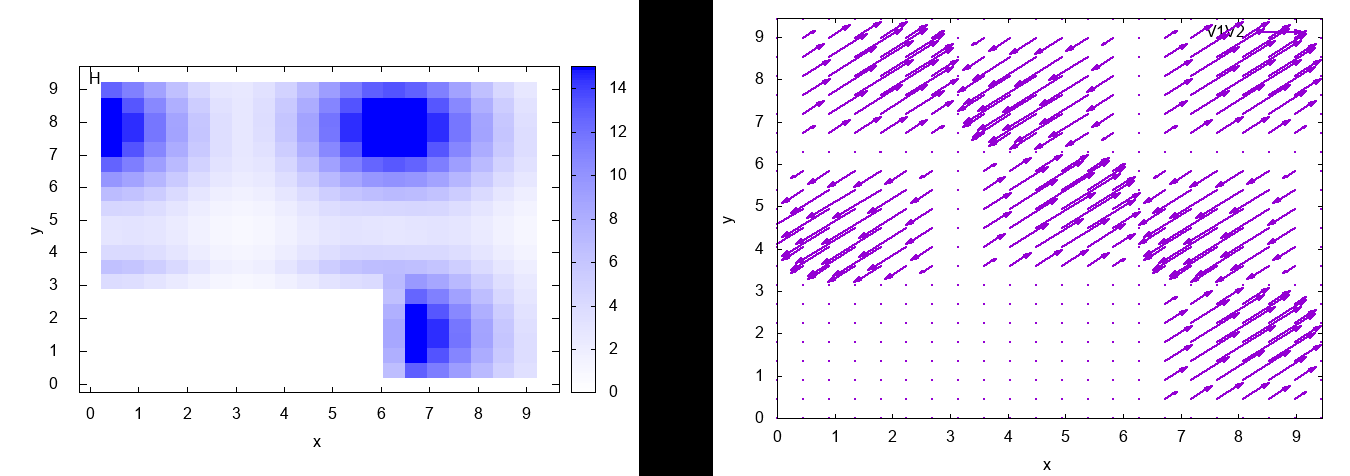
\includegraphics[width=1.0\textwidth]{cont_21.png}
\caption{N = M = 21}
\end{figure}
\begin{figure}[H]
\centering
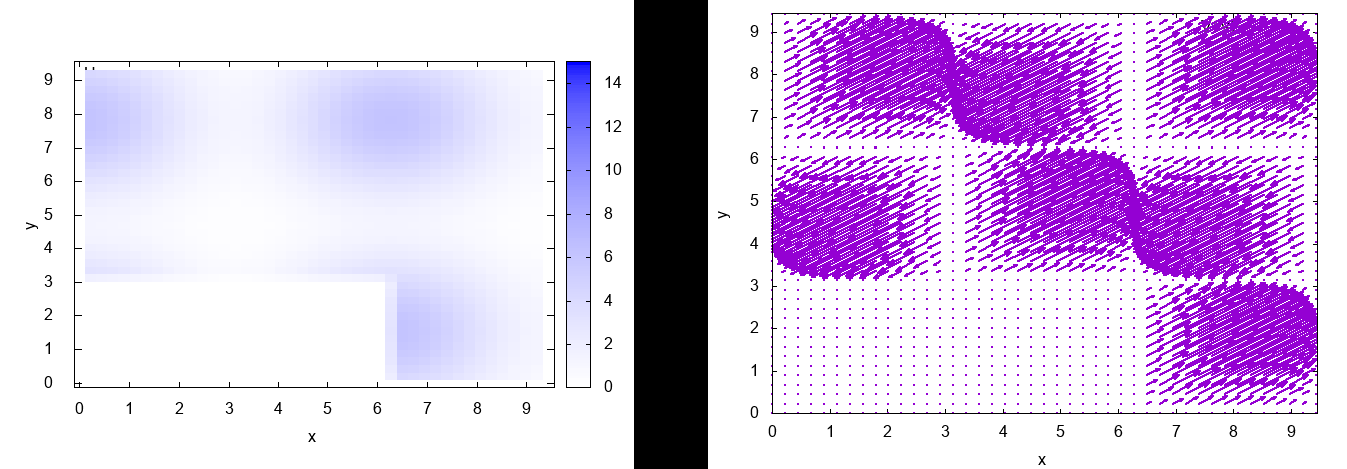
\includegraphics[width=1.0\textwidth]{cont_42.png}
\caption{N = M = 42}
\end{figure}
\begin{figure}[H]
\centering
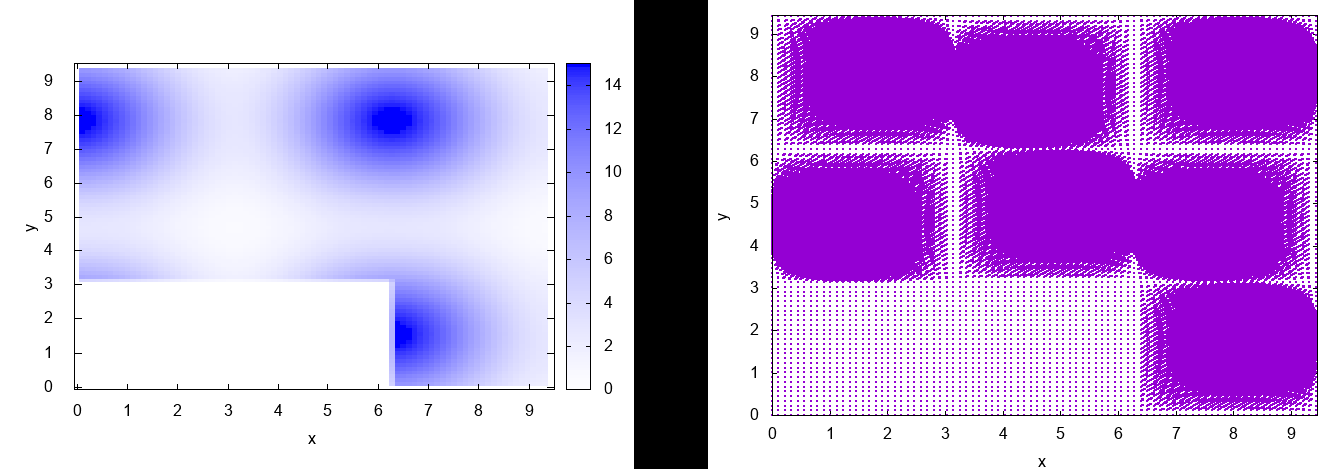
\includegraphics[width=1.0\textwidth]{cont_84.png}
\caption{N = M = 84}
\end{figure}

















\newpage
\subsection{Примеры графиков, разрывный случай}
\begin{figure}[H]
\centering
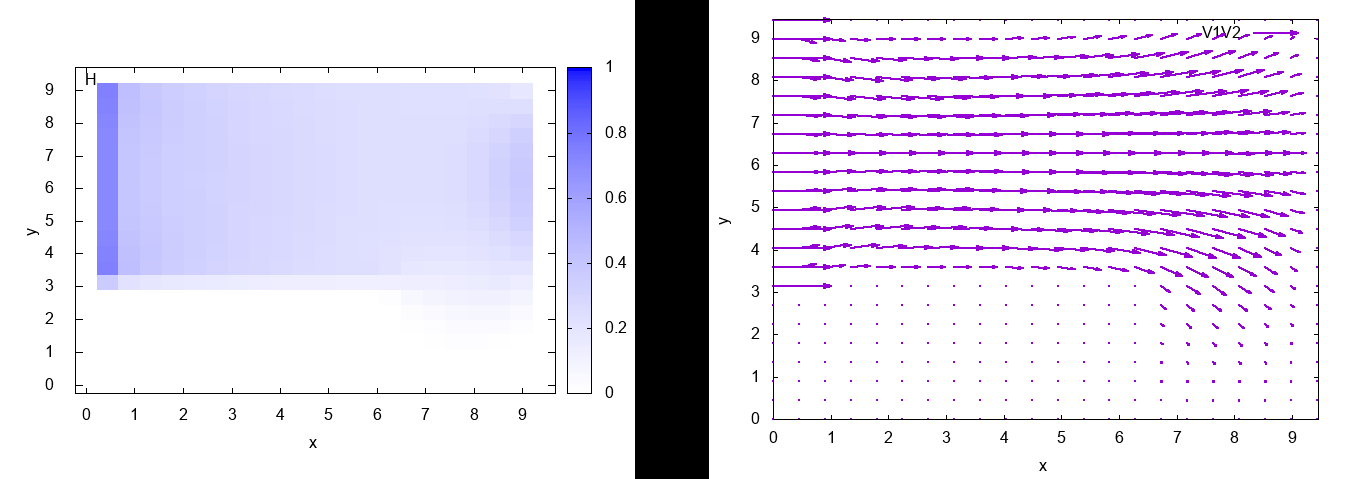
\includegraphics[width=1.0\textwidth]{discont_21.png}
\caption{N = M = 21}
\end{figure}
\begin{figure}[H]
\centering
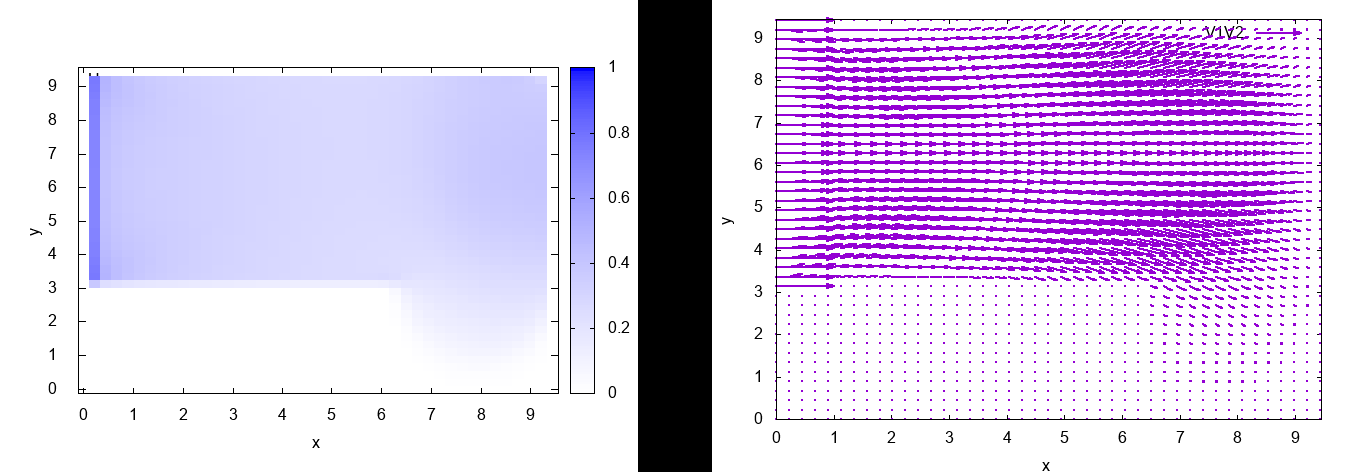
\includegraphics[width=1.0\textwidth]{discont_42.png}
\caption{N = M = 42}
\end{figure}
\begin{figure}[H]
\centering
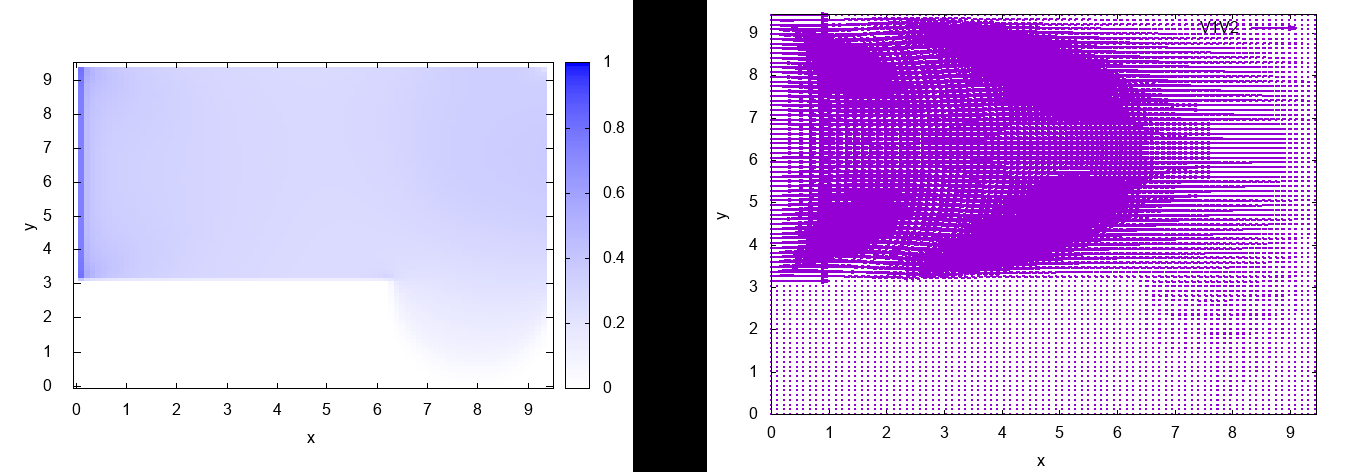
\includegraphics[width=1.0\textwidth]{discont_84.png}
\caption{N = M = 84}
\end{figure}














\section{Выводы}

Невязка в непрерывном случае, пусть сначала и является сравнительно большой, уменьшается с ожидаемой асимптотикой.
Особенно большая невязка имеется для функции плотности. Возможно, это объясняется работой с самой плотностью, а не с ее логарифмом,
поэтому ее значения оказываются достаточно большими, и по сравнению с ними невязка как раз неплохая.

В разрывном случае течение и плотность ведут себя интуитивно ожидаемым образом, поток и плотность корректно стабилизируются.

Все это позволяет думать, что схема приближения реализована корректно и работает ожидаемым образом.




\end{document}

